\documentclass[a4paper]{article} 

%% Language and font encodings
\usepackage[english]{babel}
\usepackage[utf8]{inputenc}
\usepackage[T1]{fontenc}
%% Sets page size and margins
\usepackage[a4paper,top=2cm,bottom=2cm,left=2.5cm,right=2.5cm,marginparwidth=1.75cm]{geometry}


%% Useful packages
\usepackage{amsmath}
\usepackage{graphicx}
\usepackage{tabularx}
\usepackage{xcolor}
\definecolor{tcdBlue}{RGB}{5, 105, 185}
\usepackage[colorlinks=true,allcolors=.,urlcolor=blue]{hyperref} % allowing hyperlinking of references. You can set the colour of the links or turn the colorlinks to false if no colour preferable. 
\usepackage[numbers]{natbib} % for Vancouver numbering style citation. Remove the [numbers] command for author-year Harvard style referencing. 


%% optional changes to the style. Comment (Ctrl+/) to remove these options. 
% change font to sans-serif fonts. 
\renewcommand{\familydefault}{\sfdefault}
% Format chapter headings appropriately to include tcd blue. 
\usepackage{titlesec}
\titleformat{\section}[hang]{\normalfont\Large\bfseries\color{tcdBlue}}{\thesection}{1em}{}{}


%% For nomenclature. Comment away if not used. 
% \usepackage{nomencl} % for nomenclature
% \usepackage{etoolbox} % to group nomenclature
% \usepackage{multicol} % for multiple columns in a page/table

\hyphenation{op-tical net-works semi-conduc-tor}

\begin{document}
\title{Exam report\\2024M12PY - Machine Learning with Python}
\author{Dries Luts, Bino Maiheu, Marijke Van De Steene}
\maketitle

\begin{abstract}
    This document describes the exam project for the 2024M12PY UGain course on Machine Learning with Python taught by Bart Van Rompaye.
\end{abstract}


\section{Executive summary}

A brief executive summary

\section{Analysis report}

A detailed technical description of the data analysis, training and interpretation. 

\subsection{Data analysis and processing}

In figure \ref{fig:score_histograms} we see some interesting things appear. According to \citet{bishop2006pattern}, data preprocessing is a crucial step in machine learning.

\begin{figure}
    \centering
    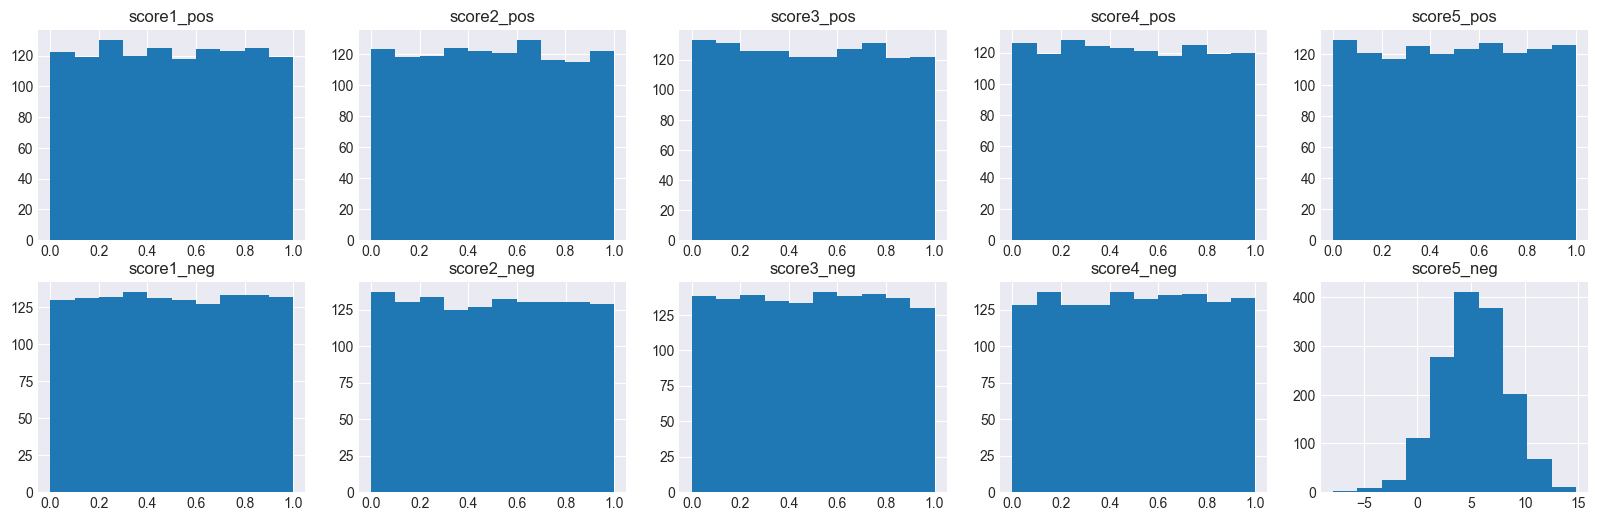
\includegraphics[width=1.0\textwidth]{figs/score_histograms.png}
    \caption{Histograms for the positivity and negativity scores by the 5 other hotels. We clearly see
    that the negativity scores for hotel 5 were not yet transformed to quantiles.}
    \label{fig:score_histograms}
\end{figure}

\subsection{Model training}


\subsection{Results and discussion}



%% References
\bibliographystyle{unsrtnat} % Vancouver reference style (numbering). 
% \bibliographystyle{agsm} % Harvard reference style (author-year). 
\bibliography{bibliography}
\addcontentsline{toc}{section}{Bibliography}

\end{document}